\section{Early Exit Neural Networks}

Early Exit Neural Networks (EENNs) are designed to provide predictions within a fixed, often reduced, inference time. 
These networks allow predictions to be made at intermediate layers, reducing the computational load and energy consumption when full-depth inference is unnecessary. 
However, this improvement in computational efficiency comes at the cost of increased memory usage, due to the added classifier layers required at various depths of the network.

Traditionally, NNs are structured as sequential stacks of layers, with predictions generated only after all layers have been processed. 
While this ensures maximal feature extraction, it introduces several limitations: high computational demand, fixed and potentially long inference time, and risk of overfitting and other inefficiencies.

EENNs address these issues by incrementally processing inputs and making early predictions once sufficient confidence is achieved. 
This is enabled by Early Exit Classifiers (EECs) which are auxiliary classifiers inserted at intermediate stages of the network. 
The original model, without these exits, is referred to as the Backbone Network.
EENNs leverage the observation that:
\begin{itemize}
    \item Many input samples can be accurately classified with shallow sub-networks.
    \item The Lottery Ticket Hypothesis suggests that smaller, well-initialized sub-networks can match the performance of deeper ones.
    \item Overthinking can degrade performance, where deeper layers can override correct early predictions.
\end{itemize}
\noindent By allowing some inputs to exit early, EENNs not only reduce inference time but may also improve accuracy in certain scenarios.

EENNs bring several advantages such as reduced inference time, less overfitting, and mitigation of vanishing gradients and overthinking. 
Notably, earlier classifiers are not necessarily less accurate than deeper one.

\paragraph*{Classifier}
Let $f_i(x)$ denote the output of an intermediate layer $i$ in the backbone network.
An EEC is added at that point to produce a prediction:
\[\bar{y}_i=C_i(f_i(x))\]
Thus, the EENNs yields a sequence of predictions $\bar{y}_1,\bar{y}_2,\dots,\bar{y}_N$, in addition to the final output $\hat{y}$.
These predictions may vary in accuracy depending on the layer at which they are computed.
\begin{figure}[H]
    \centering
    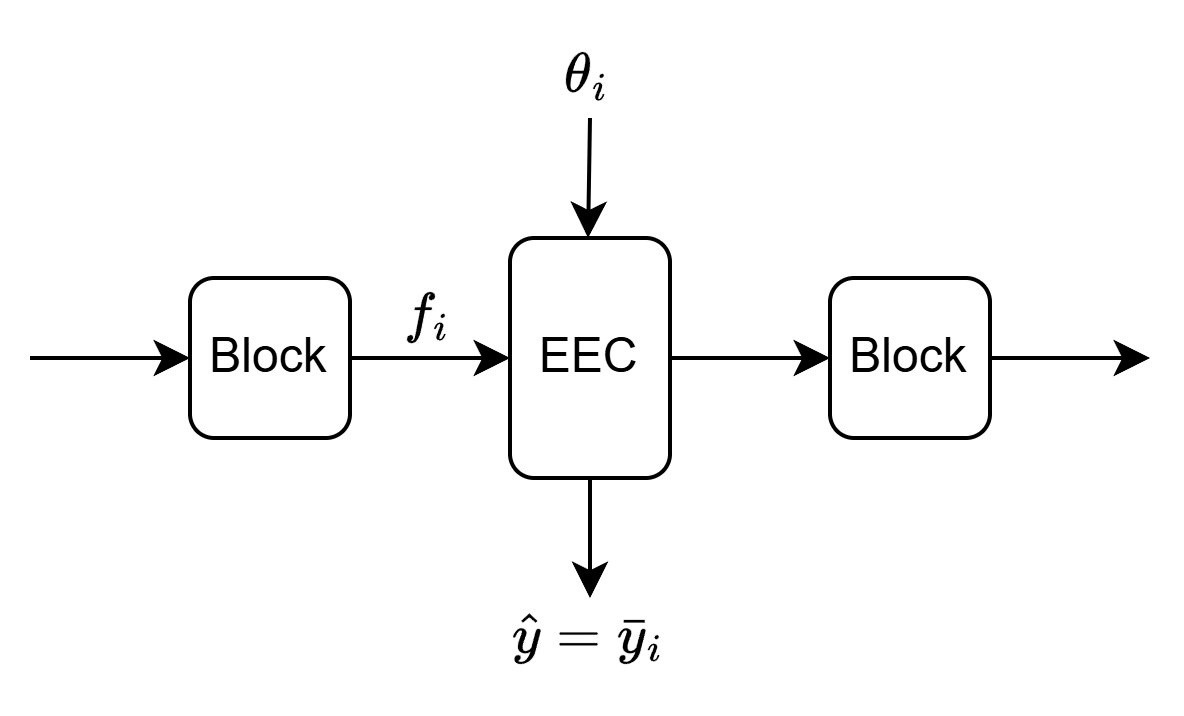
\includegraphics[width=0.5\linewidth]{images/eeai11.png}
    \caption{Early Exit Classifier}
\end{figure}

\paragraph*{Selection scheme}
To determine whether an input should exit early, each EEC is associated with a decision function governed by a threshold.
The decision function $D_i(x)$ compares the confidence score $C_i (x)$  against a predefined threshold $\theta_i$: 
\[D_i(x) = C_i (x) \geq \theta_i\]
\noindent If the confidence score exceeds the threshold, the model halts further processing and outputs $\bar{y}_i$ as the final prediction.
Otherwise, the input continues to propagate through the network.
These thresholds $\theta_i$ are key hyperparameters that control the trade-off between inference time and classification accuracy.
\begin{figure}[H]
    \centering
    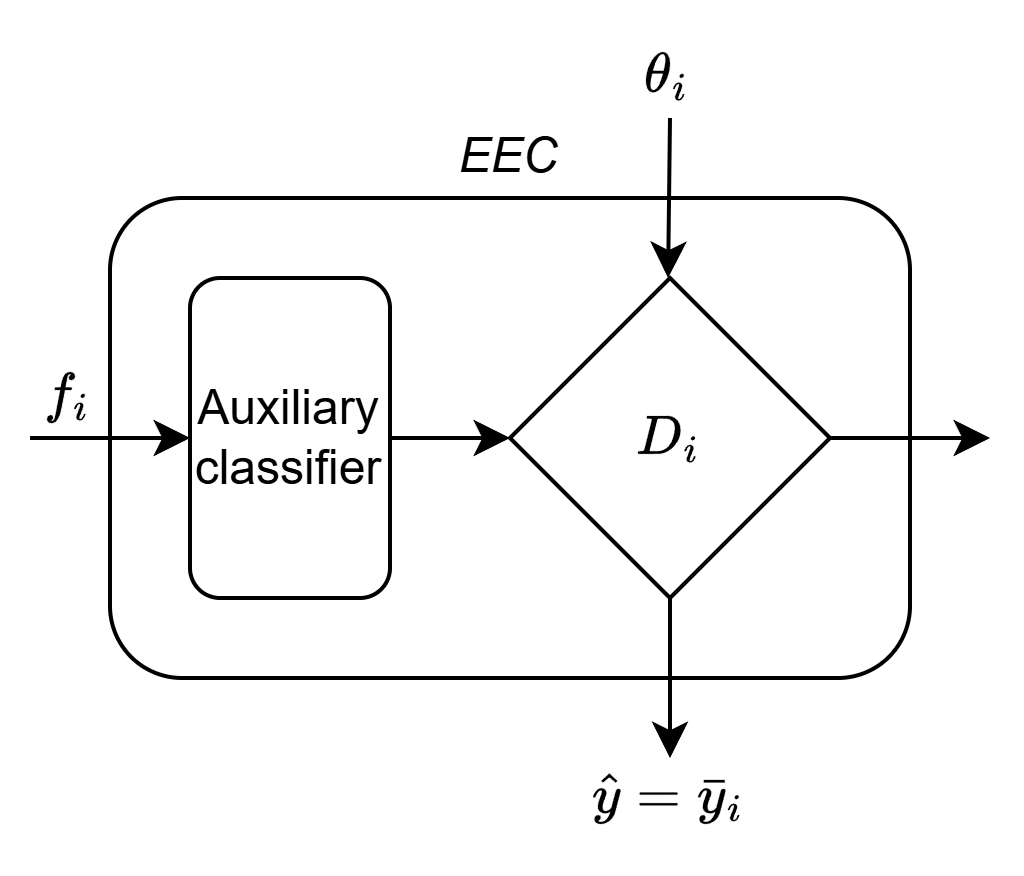
\includegraphics[width=0.4\linewidth]{images/eeai12.png}
    \caption{Early Exit Auxiliary Classifier and Decision Function}
\end{figure}
\noindent Common decision functions include:
\begin{enumerate}
    \item \textit{Maximum softmax probability}: let $S_i(x)$ be the softmax output of EEC$_i$ for input $x$. 
        The confidence is given by:
        \[\text{confidence}(x)=\max S_i(x)\]
        Here, $S_i^j(x)$ is the softmax probability for class $j$.
    \item \textit{Score margin}: defined as the difference between the top two softmax scores:
        \[\text{SM}_i=S_i^{(1)}(x)-S_i^{(2)}(x)\]
        Here, $S_i^{(1)}(x)$ and $S_i^{(2)}(x)$ are the highest and second-highest probabilities, respectively. 
        A larger margin indicates higher confidence.
    \item \textit{Entropy}: measures uncertainty in the prediction:
        \[H(y) = -\sum_{i=0}^C y_i\log(y_i)\]
        Here, $C$ is the number of classes. 
        Entropy is minimal when the output is a one-hot vector and maximal for a uniform distribution. 
\end{enumerate}

\subsection{Training}
The training of EENNs typically falls into three main strategies:
\begin{enumerate}
    \item \textit{Joint training}: in this approach, all EECs are trained simultaneously by optimizing a combined loss function:
        \[\mathcal{L}_{\text{joint}}=\mathcal{L}(\hat{y},y)+\sum_{i=1}^{N}w_i\mathcal{L}(\bar{y}_i,y)\]
        Here, $\mathcal{L}$ is the standard cross-entropy loss, $\hat{y}$ is the output of the final classifier, $\bar{y}_i$ is the output of the $i$-th EEC, $y$ is the ground truth label, $w_i$ are weighting factors, which can be uniform or treated as tunable hyperparameters, and $N$ is the total number of EECs.
    \item \textit{Layer-wise training}: this strategy trains the network progressively. 
        At each stage, a new EEC and the corresponding portion of the backbone are trained while keeping the previously trained layers frozen. 
        This approach allows the network to stabilize lower layers before deeper blocks are optimized.
    \item \textit{Knowledge distillation}: in this two-stage method, the backbone network (acting as the teacher) is trained first.
        Once trained, the EECs (students) are trained on top of the frozen backbone, learning from both the ground truth and optionally from the teacher's soft predictions.
\end{enumerate}

\subsection{Inference}
Two primary inference strategies can be adopted for EENNs:
\begin{itemize}
    \item \textit{Full evaluation}: the input is propagated through the entire network, and predictions from all EECs are aggregated to form a final decision.
    \item \textit{Early-exit inference}: the network sequentially evaluates each EEC and stops computation as soon as a confident prediction is made. 
        This enables computational savings by avoiding unnecessary processing of deeper layers.
\end{itemize}

\subsection{Architecture}
\paragraph*{BranchyNet}
BranchyNet is built on top of the original AlexNet architecture, adding two EECs at intermediate layers of the network. 
The model is trained using a joint training strategy. 
During inference, computation halts immediately once a sample meets the exit condition at an EEC, avoiding unnecessary forward propagation through deeper layers. 
The decision to exit is based on a confidence measure computed from the entropy.

\paragraph*{Gate-classification}
Gate-classification, on the other hand, take a probabilistic approach to confidence estimation. 
In these models, confidence is explicitly modeled as the posterior probability of the predicted class given the input. 
Inference proceeds sequentially through the network, and the decision to exit is made as soon as this posterior probability exceeds a predefined threshold. 